\documentclass{article}
\usepackage[utf8]{inputenc}
\usepackage[french]{babel}
\usepackage{amsmath}
\usepackage{listings}
\usepackage{hyperref}
\usepackage{xcolor}
\usepackage{graphicx}
\usepackage[style=authoryear]{biblatex}
\usepackage{fancyhdr}
\usepackage{braket}
\usepackage{float}
\usepackage{color}
\usepackage{tabularx}

\definecolor{codegreen}{rgb}{0,0.6,0}
\definecolor{codegray}{rgb}{0.5,0.5,0.5}
\definecolor{codepurple}{rgb}{0.58,0,0.82}
\definecolor{backcolour}{rgb}{0.95,0.95,0.92}

\lstdefinestyle{mystyle}{
  backgroundcolor=\color{backcolour},   
  commentstyle=\color{codegreen},
  keywordstyle=\color{magenta},
  numberstyle=\tiny\color{codegray},
  stringstyle=\color{codepurple},
  basicstyle=\ttfamily\footnotesize,
  breakatwhitespace=false,         
  breaklines=true,                 
  captionpos=b,                    
  keepspaces=true,                 
  numbers=left,                    
  numbersep=5pt,                  
  showspaces=false,                
  showstringspaces=false,
  showtabs=false,                  
  tabsize=2
}

\pagestyle{fancy}

\fancyhf{}
\fancyhead[L]{Rapport de projet : PythQuest}
\fancyhead[R]{RAETH et SANNA, L3STI}
\fancyfoot[C]{Page n°\thepage}
\fancyfoot[L]{Université de Corse}
\fancyfoot[R]{
\includegraphics[height=1cm]{img/univCorse.png}}

\addbibresource{ref.bib}

\title{Rapport de séminaire :\\L'algorithme quantique}
\author{Léandre RAETH, Thomas SANNA\\L3 Sciences et Technologies, Parcours Informatique}
\date{\today}

\begin{document}

\begin{titlepage}
  \begin{center}
      
\includegraphics[width=0.5\textwidth]{img/univCorse.png}\\[1cm]
      
      \textsc{\LARGE Université de Corse}\\[1.5cm]
      
      \textsc{\Large Année universitaire 2024-2025}\\[0.5cm]
      
      \vfill
      
      \hrulefill\\[0.4cm]
      {\Huge \bfseries Rapport de Projet}\\[0.4cm]
      \hrulefill\\[0.4cm]
      
      \textsc{\Large PythQuest }\\[0.5cm]
      
      \vfill
      
      \textbf{Présenté par :}\\
      Léandre RAETH, Thomas SANNA\\
      
      \vfill
      
      \textbf{Projet présenté le 05/04/2025}\\
      \vfill
      
      \textsc{L3 Sciences et Technologies, Parcours Informatique}
      
  \end{center}
\end{titlepage}

\break\tableofcontents

\break\section{Introduction}
\subsection{Présentation du projet}

PythQuest est un jeu de rôle textuel développé en Python, conçu dans le cadre du projet de fin de semestre. Ce jeu met en œuvre une architecture MVC (Modèle-Vue-Contrôleur) pour séparer la logique métier, l'interface utilisateur et la gestion des interactions. 

Le joueur incarne un aventurier qui doit accomplir des quêtes, explorer des donjons, combattre des monstres et gérer son inventaire pour progresser dans le jeu. Les principales fonctionnalités incluent :
\begin{itemize}
    \item \textbf{Gestion des quêtes} : Le joueur peut accepter des quêtes, les accomplir en battant des monstres spécifiques, et recevoir des récompenses en or et en expérience.
    \item \textbf{Exploration de donjons} : Les donjons contiennent des monstres aléatoires que le joueur peut combattre pour gagner des ressources.
    \item \textbf{Système de combat} : Le joueur peut attaquer les monstres, utiliser des potions pour se soigner, ou fuir les combats.
    \item \textbf{Gestion de l'inventaire} : Le joueur peut consulter ses armes, potions et équipements, et choisir une arme à équiper.
    \item \textbf{Interactions avec des PNJ} : Le joueur peut acheter des armes auprès d'un forgeron ou des potions auprès d'un médecin.
\end{itemize}

\subsection{Déroulement du jeu}
Le joueur crée se compte, ou se connecte avec son email et son mot de passe. Son personnage est alors créé à la suite de l'entrée de son nom.

Le joueur commence niveau 1. Son objectif est de monter de niveau en accomplissant des quêtes créees aléatoirement par le jeu.

Les quêtes consistent à battre un monstre spécifique qui se trouve dans un donjon regroupant plusieurs autres monstres aléatoires. Le joueur peut choisir de combattre ces monstres pour gagner de l'or et de l'expérience, ou de fuir.

Lors de l'entrée d'un donjon, des monstres apparaissent aléatoirement à tour de rôle. Le joueur peut choisir d'attaquer, de fuir ou d'utiliser une potion pour se soigner. S'il choisit d'attaquer, il peut infliger des dégâts au monstre et recevoir des coups en retour, selon l'arme qu'équipe le monstre face à lui.

Lorsqu'un monstre est vaincu, le joueur gagne de l'expérience, de l'or, et parfois une arme que le monstre possédait. Si le monstre vaincu est celui requis pour une quête en cours, la quête est marquée comme terminée, et le joueur reçoit une récompense supplémentaire en or et en expérience.

Si le joueur subit trop de dégâts et que ses points de vie tombent à zéro, il est renvoyé au village. Dans ce cas, il perd une partie de son or et doit se soigner ou acheter des potions auprès du médecin pour continuer son aventure.

Le joueur peut également interagir avec des PNJ (personnages non-joueurs) dans le village :
\begin{itemize}
    \item \textbf{Le forgeron} : Permet d'acheter ou de vendre des armes, et parfois de forger de nouvelles armes.
    \item \textbf{Le médecin} : Vend des potions de soin pour restaurer les points de vie du joueur.
\end{itemize}

Le jeu propose une progression basée sur le niveau du joueur. À chaque montée de niveau, le joueur devient plus puissant, ce qui lui permet d'affronter des donjons et des monstres de plus grande difficulté. Les quêtes et les récompenses s'adaptent également au niveau du joueur, offrant un défi constant.

Il n'y a pas d'objectif final à proprement parler. Le joueur gagne du niveau à l'infini, et il y aura toujours des quêtes à faire au fil de l'aventure.

\section{Conception orientée objet}

\subsection{Classes Principales}

Le projet PythQuest repose sur une conception orientée objet, avec une organisation en plusieurs classes principales pour modéliser les différents éléments du jeu. Voici un aperçu des classes principales :

\begin{itemize}
    \item \textbf{Personnage} : Classe de base représentant un personnage dans le jeu. Elle contient des attributs communs tels que le nom, les points de vie et l'or. Les classes spécifiques comme \textit{Combattant}, \textit{Monstre}, \textit{Forgeron} et \textit{Médecin} héritent de cette classe.
    
    \item \textbf{Combattant} : Représente le joueur. Cette classe gère les actions du joueur, telles que l'attaque, l'utilisation de potions, la gestion de l'inventaire, et l'accomplissement des quêtes. Elle contient également des attributs comme le niveau, l'expérience, et l'arme équipée.
    
    \item \textbf{Monstre} : Représente les ennemis que le joueur peut combattre dans les donjons. Chaque monstre possède un niveau, des points de vie, une arme, et une récompense en or.
    
    \item \textbf{Quête} : Modélise les quêtes que le joueur peut accepter. Une quête est associée à un monstre cible, un donjon, une difficulté, et une récompense en or. Elle contient également un statut indiquant si la quête est en cours ou terminée.
    
    \item \textbf{Donjon} : Représente les donjons explorables par le joueur. Chaque donjon contient une liste de monstres et est associé à un niveau de difficulté.
    
    \item \textbf{Arme} : Représente les armes que le joueur ou les monstres peuvent utiliser. Chaque arme a un nom, des dégâts, et une valeur en or.
    
    \item \textbf{Forgeron} : PNJ permettant au joueur d'acheter, de vendre ou de forger des armes. Il gère également un stock d'armes disponibles.
    
    \item \textbf{Médecin} : PNJ permettant au joueur d'acheter des potions pour restaurer ses points de vie. Il gère un stock limité de potions.
    
    \item \textbf{GestionnaireDeQuêtes} : Classe utilitaire responsable de la création et de la gestion des quêtes. Elle génère des quêtes aléatoires adaptées au niveau du joueur.
\end{itemize}

Chaque classe est conçue pour être modulaire et réutilisable, avec des méthodes spécifiques pour gérer les interactions entre les différents éléments du jeu, et leur création.

\begin{figure}[H]
    \centering
    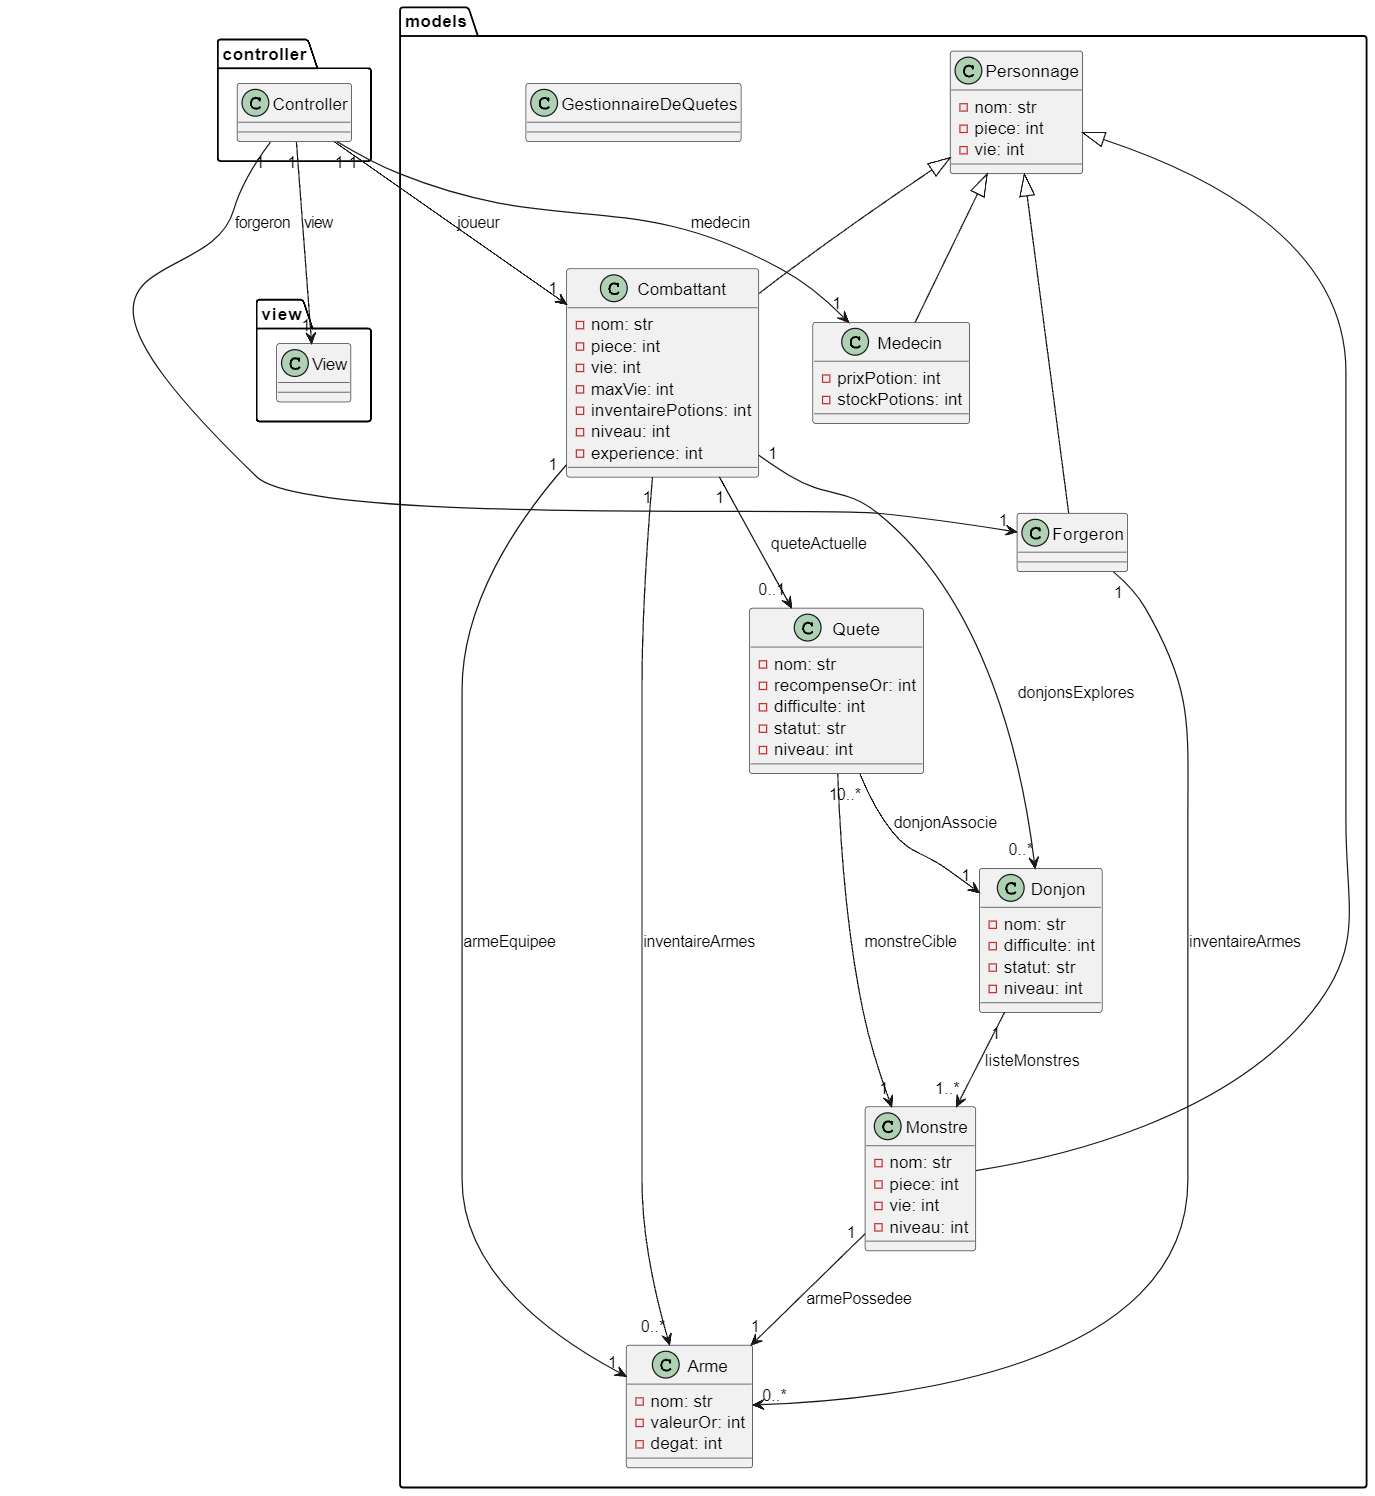
\includegraphics[width=1\textwidth]{img/UML.png}
    \caption{Diagramme UML du projet PythQuest sans DAO}
    \label{fig:diagramme_classes}
\end{figure}

\subsection{Cas d'utilisation principaux}

Voici les principaux cas d'utilisation du jeu PythQuest :

\begin{itemize}
    \item \textbf{Créer un personnage} : Le joueur peut créer un nouveau personnage en entrant son nom, son email et son mot de passe. Une fois créé, le personnage commence au niveau 1 avec un équipement de base.

    \item \textbf{Accepter une quête} : Le joueur peut consulter les quêtes disponibles et en accepter une. Chaque quête est associée à un monstre spécifique à vaincre et offre des récompenses en or et en expérience.

    \item \textbf{Explorer un donjon} : Le joueur peut entrer dans un donjon pour affronter des monstres aléatoires. Chaque donjon est associé à un niveau de difficulté et contient des monstres adaptés au niveau du joueur.

    \item \textbf{Combattre un monstre} : Lors d'une exploration de donjon, le joueur peut engager un combat avec un monstre. Il peut choisir d'attaquer, d'utiliser une potion pour se soigner ou de fuir.

    \item \textbf{Acheter des armes} : Le joueur peut interagir avec le forgeron pour acheter de nouvelles armes, vendre des armes inutilisées ou forger des armes plus puissantes.

    \item \textbf{Acheter des potions} : Le joueur peut interagir avec le médecin pour acheter des potions de soin afin de restaurer ses points de vie.

    \item \textbf{Gérer l'inventaire} : Le joueur peut consulter son inventaire pour voir les armes et potions qu'il possède. Il peut également équiper une arme pour l'utiliser en combat.

    \item \textbf{Sauvegarder et charger une partie} : Le joueur peut sauvegarder sa progression lors de sa déconnexion et la charger ultérieurement pour continuer son aventure à sa connexion.

    \item \textbf{Abandonner une quête} : Si le joueur ne souhaite plus poursuivre une quête en cours, il peut l'abandonner pour en choisir une autre.
\end{itemize}


\section{Technologies utilisées}

Le projet a été développé en Python (d'où le nom PythQuest), en utilisant la bibliothèque Tkinter pour l'interface graphique, et mysql pour la gestion de la base de données.

Le code est organisé selon le modèle MVC (Modèle-Vue-Contrôleur) pour une meilleure séparation des préoccupations. Le modèle gère la logique métier et les données, la vue s'occupe de l'interface utilisateur, et le contrôleur gère les interactions entre le modèle et la vue.

Le code est structuré et vérifié à ce que les classes soient bien séparées et que les méthodes soient cohérentes. Des commentaires sont présents pour expliquer le fonctionnement de certaines parties du code.

\subsection{Nos bonnes pratiques}

Ce projet suit plusieurs bonnes pratiques de codage pour garantir la maintenabilité, la lisibilité et la robustesse du code. Voici les principales pratiques adoptées :

\begin{itemize}
    \item \textbf{Nommage des variables et des fonctions} :
    \begin{itemize}
        \item Utilisation de noms explicites et significatifs pour les variables et les fonctions.
        \item Adoption du style \textit{camelCase} pour les noms de variables et de fonctions (ex : \texttt{nomDeVariable}, \texttt{nomDeFonction}).
        \item Utilisation du style \textit{PascalCase} pour les noms de classes (ex : \texttt{NomDeClasse}).
        \item Utilisation du style \textit{snake\_case} pour les noms de constantes (ex : \texttt{NOM\_DE\_CONSTANTE}).
        \item Éviter les noms de variables génériques comme \texttt{x}, \texttt{y}, \texttt{temp}, etc.
    \end{itemize}

    \item \textbf{Structure du code} :
    \begin{itemize}
        \item Séparation de la logique applicative et de l'interface utilisateur grâce au modèle MVC (Modèle-Vue-Contrôleur).
        \item Organisation du code en modules et fichiers logiques.
        \item Documentation des classes, méthodes et fonctions à l'aide de \textit{docstrings}.
        \item Utilisation de constantes pour éviter les valeurs en dur dans le code.
    \end{itemize}

    \item \textbf{Structure MVC} :
    \begin{itemize}
        \item Le modèle (\textit{Model}) contient la logique métier et les données.
        \item La vue (\textit{View}) gère l'affichage et l'interface utilisateur.
        \item Le contrôleur (\textit{Controller}) gère les interactions entre le modèle et la vue.
        \item Éviter de mélanger la logique métier avec l'interface utilisateur.
        \item Regrouper tout ce qui concerne une classe dans le même fichier (ex : \texttt{Combattant} dans \texttt{models/combattant.py}).
        \item Organisation des fichiers : les classes de modèles dans \texttt{models/}, les classes de vues dans \texttt{view/}, et les classes de contrôleurs dans \texttt{controller/}.
    \end{itemize}

    \item \textbf{Gestion des exceptions} :
    \begin{itemize}
        \item Gestion appropriée des exceptions pour éviter les plantages inattendus.
        \item Création d'exceptions personnalisées pour les erreurs spécifiques à l'application (dans \texttt{models/exceptions.py}).
        \item Utilisation de blocs \texttt{try-except} pour capturer et gérer les erreurs spécifiques.
    \end{itemize}

    \item \textbf{Tests automatisés} :
    \begin{itemize}
        \item Écriture de tests unitaires pour vérifier le bon fonctionnement des différentes parties du code.
        \item Utilisation de frameworks de test comme \texttt{unittest} ou \texttt{pytest} pour automatiser les tests.
    \end{itemize}

    \item \textbf{Documentation} :
    \begin{itemize}
        \item Documentation du code avec des commentaires et des \textit{docstrings}.
        \item Utilisation d'annotations de type pour spécifier les types de paramètres et de retour des fonctions.
        \item Maintien d'un fichier \texttt{README} à jour avec des instructions claires pour l'installation et l'utilisation du projet.
    \end{itemize}
\end{itemize}


\section{Structuration du code : MVC}

Comme expliqué précédemment, le projet est structuré selon le modèle MVC (Modèle-Vue-Contrôleur). Voici un aperçu de la structure du code :

\begin{figure}[H]
    \centering
    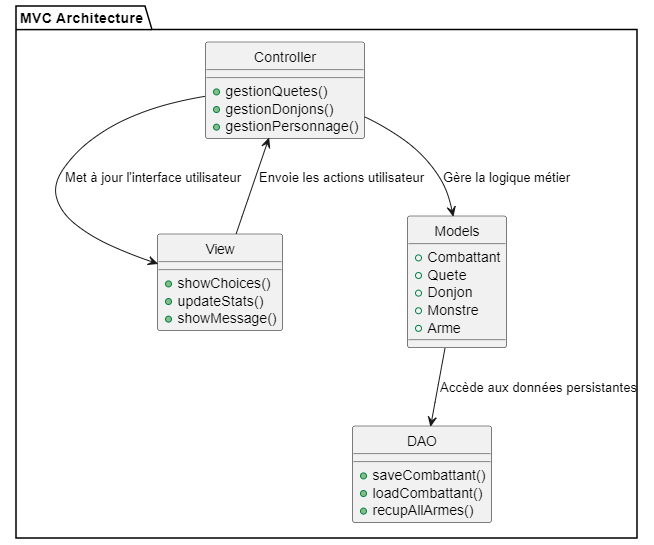
\includegraphics[width=1\textwidth]{img/MVC.png}
    \caption{Structure du code selon le modèle MVC}
    \label{fig:mvc_structure}
\end{figure}

\section{Base de données}

PythQuest est un jeu pensé hors-ligne. Mais nous avons tout de même implémenté une base de données sur un serveur et non en local, pour nous permettre une compréhension de la gestion des bases de données en Python.

En conséquence que le jeu soit hors-ligne, aucune donnée d'un joueur n'interfère avec un autre joueur. Chaque joueur possède ses propres armes, son forgeron, etc\dots

Voici donc le "Concepteur" de base de données :

\begin{figure}[H]
    \centering
    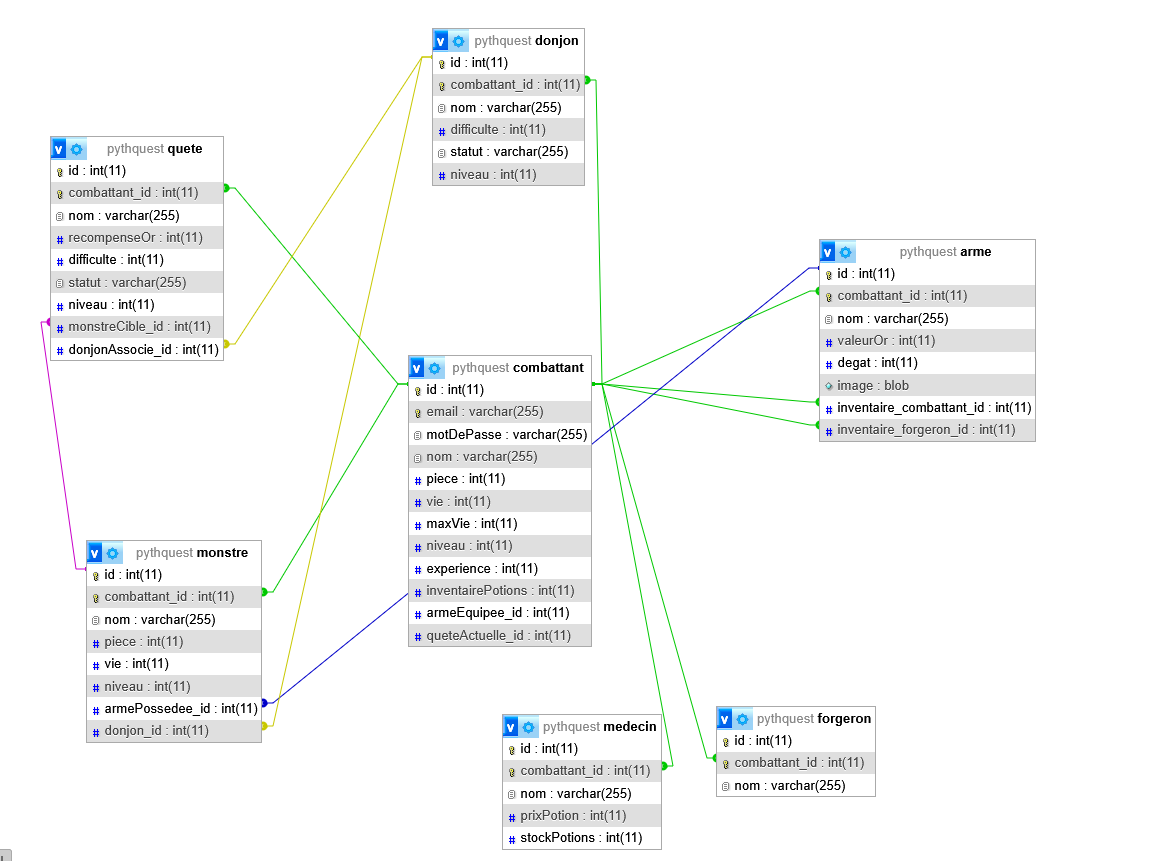
\includegraphics[width=1\textwidth]{img/BDD.png}
    \caption{Concepteur de la base de données}
    \label{fig:base_de_donnees}
\end{figure}

En effet, on peut voir que l'unicité d'un élément d'une table, par exemple "arme", est gérée par l'ID de l'arme, mais aussi par l'id du joueur. 

Cela permet de s'assurer qu'aucun joueur n'aura la même arme qu'un autre joueur.


\section{Interface graphique}

L'interface graphique du jeu a été développée à l'aide de la bibliothèque Tkinter. Elle permet d'interagir avec le joueur de manière intuitive et agréable. Voici un aperçu de la fenêtre principale du jeu :

\begin{figure}[H]
    \centering
    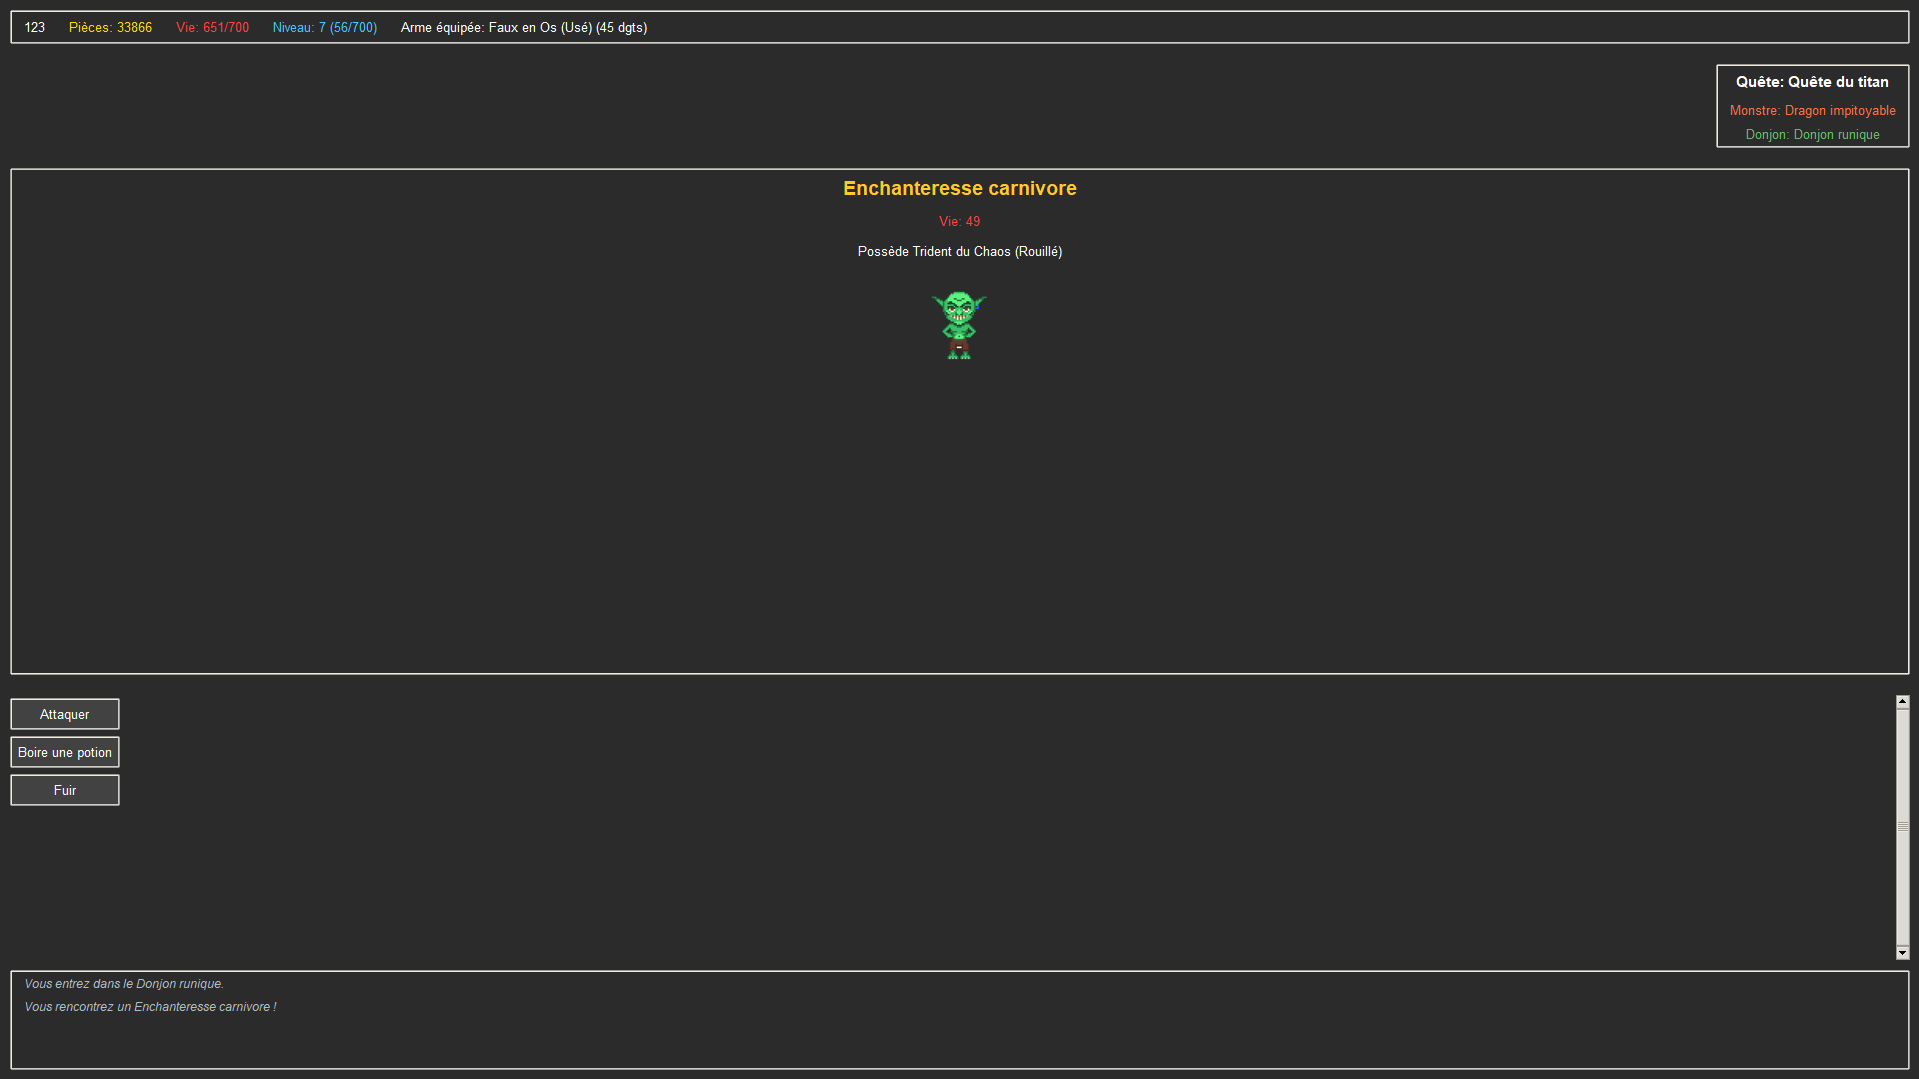
\includegraphics[width=1\textwidth]{img/fenetre.png}
    \caption{Fenêtre principale du jeu}
    \label{fig:interface_graphique}
\end{figure}

\begin{figure}[H]
  \centering
  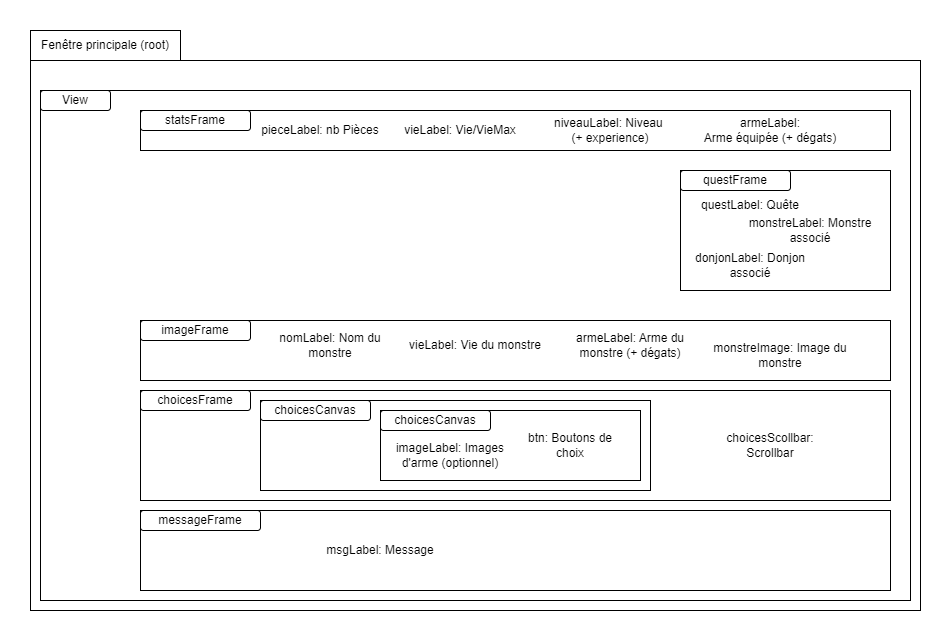
\includegraphics[width=1\textwidth]{img/uiSchem.png}
  \caption{Structure de l'interface du jeu}
  \label{fig:interface_graphique}
\end{figure}


\section{Suivi de projet}

\subsection{Gestion de projet}
Le projet a été géré de manière collaborative, avec une répartition des tâches entre les membres de l'équipe. Nous avons utilisé un système de gestion de version (Git) pour suivre les modifications du code et faciliter la collaboration. Nous avons également utilisé Discord pour prévenir de certains changements et les expliquer.

\subsection{Lien du dépôt Git}

Le code source du projet est disponible sur GitHub. Vous pouvez y accéder en suivant ce lien : 
\href{https://github.com/ThomasSanna/projet-POO-L3STI}{https://github.com/ThomasSanna/projet-POO-L3STI}

Voici les différentes branches du projet :
\begin{itemize}
  \item \textbf{V1} : Version 1.0 du projet
  \item \textbf{V2} : Version 2.0 du projet
  \item \textbf{V3} : Version 3.0 du projet
  \item \textbf{VFinale} : Version finale du projet
  \item \textbf{Main} : Version principale du projet, qui est la version 4.0 du projet. Cette branche n'a contenu que des versions fonctionnelles. Si une version ne fonctionnait pas, elle était mise dans une autre branche.
  \item \textbf{Thomas} : Branche de Thomas, qui a été utilisée pour le développement de certaines fonctionnalités du jeu.
  \item \textbf{Leandre} : Branche de Léandre, qui a été utilisée pour le développement de certaines fonctionnalités du jeu, et pour la gestion de l'UI
  \item \textbf{UIThomas} : Branche de Thomas, qui a été utilisée pour le développement de l'UI du jeu.
  \item \textbf{ThomasConn} : Branche de Thomas, qui a été utilisée pour le développement de la connexion du jeu et des sauvegardes.
\end{itemize}



\subsection{Versions du projet}

Le projet a été développé en 4 versions principales, chacune correspondant à une étape clé de son développement. Voici un aperçu des principales versions et des fonctionnalités ajoutées à chaque étape :

\begin{itemize}
    \item \textbf{Version 1.0} : Création de la structure de base du projet, avec les classes principales (Personnage, Combattant, Monstre, Quête, Donjon, Arme). Mise en place des premières fonctionnalités de jeu sous forme vue console.
    
    \textit{Toute cette version a été fait en Pair Programming. Léandre a souvent pris le rôle du "Navigateur" (celui qui propose des idées et des solutions), tandis que Thomas a pris le rôle du "Conducteur" (celui qui tape le code). Nous avons alterné ces rôles au fil du projet, mais nous avons souvent gardé cette répartition.}
    \begin{itemize}
        \item Gestion de quêtes (acceptation, accomplissement, abandon)
        \item Exploration de donjons
        \item Combat contre des monstres
        \item Gestion de l'expérience et des niveaux
        \item Gestion de l'inventaire et de l'equipement d'arme
        \item Gestion de l'or et des récompenses lors d'une fin de quête ou d'une victoire contre un monstre
        \item Gestion de la mort du joueur et pénalisation de l'or
    \end{itemize}
    
    \item \textbf{Version 2.0} : 
    
    \textit{Nous nous sommes attribués des tâches à faire chacun de note côté. Pour chaque cas ci-dessous, les informations sur qui a fait quoi sont indiquées, avec informations supplémentaires.}
    \begin{itemize}
      \item Ajout de commentaires et de docstrings pour améliorer la lisibilité du code. [Thomas]
      \item Mise en place du systeme MVC pour séparer la logique métier et l'interface utilisateur à l'aide d'un contrôleur. [Thomas]
      \item Ajout de l'interface graphique avec Tkinter pour améliorer l'expérience utilisateur. [Léandre. Avec l'aide de Thomas pour lier au contrôleur]
      \item Création aléatoire des quêtes et des monstres dans les donjons. [Thomas]
      \item Ajout de la gestion des niveaux de difficulté des quêtes et des monstres. [Thomas]
      \item Implémentation du forgeron et achat d'arme [Thomas]
      \item Implémentation du médecin et achat de potions [Thomas]
      \item Ajout d'images personnalisées pour les armes. [Léandre]
    \end{itemize}
    
    \item \textbf{Version 3.0} :
    
    \textit{Nous avons continué à nous répartir les tâches.}
    \begin{itemize}
      \item Ajout de tests unitaires pour valider le bon fonctionnement de la classe Combattant et de certaines de ses méthodes. [Thomas]
      \begin{itemize}
        \item gagnerExperience
        \item resetApresMort
        \item gagnerPotion
        \item perdrePotion
        \item boirePotion
        \item acheterPotion
        \item acheterArme
        \item accepterQuete
        \item abandonnerQuete
        \item battreMonstre
        \item attaquer
      \end{itemize}
      \item Implémentation de la base de données [Thomas]
      \item Ajout de la gestion de la connexion et de la création de compte (Combattant et son inventaire d'armes et potions) [Thomas]
      \item Ajout de la gestion de la sauvegarde et du chargement de la partie (Combattant et son inventaire d'armes et potions) [Thomas]
    \end{itemize}
    
    
    \item \textbf{Version Finale} : Optimisation du code et ajout de commentaires pour améliorer la lisibilité. Tests finaux et corrections de bugs. Préparation du rapport final.
\end{itemize}

\subsection{Corrections mineures, corrections de bugs}
Le projet a été testé tout au long de son développement, et plusieurs bugs ont été corrigés. Voici quelques exemples de bugs identifiés et corrigés :

\begin{itemize}

  \item \textbf{Version 1.0 $\rightarrow$ Version 2.0} :
  \begin{itemize}
    \item Correction du fait que le joueur pouvait battre un monstre qui appartenait à une quête non-associée, sans que la quête ne soit notée comme "Terminée".
    \item Optimisation de la création de donjon :
    \begin{itemize}
      \item Empêcher la création d'un donjon qui possède la même difficulté qu'un donjon déjà en cours.
    \end{itemize}
    \item Correction du fait que le combat contre un monstre d'une quête associée ne se terminait pas correctement.
    \item Affichage de la récompense en or de la quête, ainsi que l'affichage de la récompense d'arme et d'or lorsqu'on bat un monstre.
    \item Correction du fait que le joueur n'arrivait pas à fuir un donjon.
    \item Correction du fait que le joueur pouvait avoir une valeur négative d'expérience lors d'un passage de niveau.
    \item Correction de certaines méthodes dans Forgeron et Combattant qui utilisaient encore des print() pour afficher des informations.
  \end{itemize}

  \item \textbf{Version 2.0 $\rightarrow$ Version 3.0} :
  \begin{itemize}
    \item Correction du fait que les données sur l'écran ne se mettaient pas à jour lors d'un certain cas à l'achat de potion et de vie.
    \item Ajout du nom du joueur dans l'interface graphique.
    \item Ajout de plusieurs icones pour représenter les monstres lors d'un combat.
  \end{itemize}

  \item \textbf{Version 3.0 $\rightarrow$ Version Finale} :
  \begin{itemize}
    \item
  \end{itemize}

\end{itemize}

\subsection{Rééquilibrage du jeu}
Pour qu'un jeu soit appréciable, il faut impérativement qu'il soit équilibré.

\begin{itemize}

  \item \textbf{Version 1.0 $\rightarrow$ Version 2.0} :
  \begin{itemize}
    \item Baisse de la récompense d'or des monstres de $~20\%$.
    \item Baisse des dégâts des monstres ($3 \text{ à } 10 \to 2 \text{ à } 5$ (évoluant avec la difficulté et le niveau du joueur)).
    \item Baisse de la vie maximale obtenue lors d'un passage de niveau, qui était beaucoup trop élevée au fil du temps ($VieMax \cdot 1.5$ $\to$ $VieMax + 100$ à chaque niveau).
    \item Augmentation du prix des armes chez le forgeron de $~50\%$.
  \end{itemize}

  \item \textbf{Version 2.0 $\rightarrow$ Version 3.0} :
  \begin{itemize}
    \item Baisse de la scalabilité des dégâts des monstres selon le niveau du joueur ($\text{Dégâts} \cdot \text{niveau} \to \text{Dégâts} \cdot \sqrt{\text{niveau}}$).
    \item Baisse de la scalabilité des dégâts des monstres selon la difficulté du donjon ($\text{Dégâts} \cdot \text{difficulté} \to \text{Dégâts} \cdot \sqrt{\text{difficulté}}$).
    \item Baisse de la scalabilité de l'or des monstres selon le niveau du joueur ($\text{Or} \cdot \text{niveau} \to \text{Or} \cdot \sqrt{\text{niveau}}$).
  \end{itemize}

  \item \textbf{Version 3.0 $\rightarrow$ Version Finale} :
  \begin{itemize}
    \item Ajout d'un multiplicateur de vie rendu d'une potion selon le niveau du joueur. ($GAIN\_POTION \to GAIN\_POTION \cdot \sqrt{\text{niveau}}$).
  \end{itemize}
  
\end{itemize}

\section{Conclusion}

\subsection{Ce qu'on a appris}

Nous avons appris pas mal de chose durant la création de ce projet, dont l'utilisation des branches git, la gestion de base de données en Python (qui est sensiblement la même que pour le PHP), la gestion de l'UI en Python, ainsi que la compréhension plus approfondie de la structure MVC avec DAO, et la gestion de projet en général.

\subsection{Ce qu'on aurait pu faire différemment}

Nous aurions pu mieux préparer les présentations en amont : Rendre lisible le code et faire un rapport plus détaillé.

\subsection{Nos difficultés}

Par manque de temps, de baisse de motivation, ou même l'augmentation d'un stress au fil des différentes présentations et UE, notre projet est sans doute loin d'être parfait.

Nous avons eu du mal à garder une certaine régularité dans le travail. Certaines fonctionnalités n'ont pas vu le jour au détriment d'autres plus importantes.

Nous avons eu du mal à gérer le temps de travail, et nous aurions pu mieux nous organiser, avec l'envoi de message (ou suivi git) lors du commencement d'une tâche, et d'un indice de temps avant la fin de celle-ci.


\end{document}